\documentclass[tikz,border=8pt]{standalone}
% Shared look for every TikZ diagram. Load with % Shared look for every TikZ diagram. Load with % Shared look for every TikZ diagram. Load with \input{../../tools/tikz-style.tex}
\usepackage[T1]{fontenc}
\usepackage{lmodern}
\renewcommand{\sfdefault}{lmr}  % diagrams use the same serif as the text
\usetikzlibrary{arrows.meta, positioning, shapes.geometric, calc, fit, backgrounds}
\definecolor{cblue}{HTML}{4C78A8}
\definecolor{corange}{HTML}{F58518}
\definecolor{cgreen}{HTML}{54A24B}
\definecolor{cred}{HTML}{E45756}
\definecolor{cpurple}{HTML}{B279A2}
\definecolor{cgrey}{HTML}{6B6B6B}
\tikzset{
  every picture/.style={font=\sffamily, line width=1.2pt},
  box/.style={draw=#1, fill=#1!12, rounded corners=4pt, align=center, inner sep=7pt, minimum height=1.1cm},
  box/.default=cgrey,
  arrow/.style={-{Stealth[length=3mm]}, draw=cgrey, line width=1.4pt},
  title/.style={font=\sffamily\bfseries\Large},
  note/.style={font=\sffamily\small, text=cgrey, align=center},
}
\AtBeginDocument{\hyphenpenalty=10000 \exhyphenpenalty=10000}

\usepackage[T1]{fontenc}
\usepackage{lmodern}
\renewcommand{\sfdefault}{lmr}  % diagrams use the same serif as the text
\usetikzlibrary{arrows.meta, positioning, shapes.geometric, calc, fit, backgrounds}
\definecolor{cblue}{HTML}{4C78A8}
\definecolor{corange}{HTML}{F58518}
\definecolor{cgreen}{HTML}{54A24B}
\definecolor{cred}{HTML}{E45756}
\definecolor{cpurple}{HTML}{B279A2}
\definecolor{cgrey}{HTML}{6B6B6B}
\tikzset{
  every picture/.style={font=\sffamily, line width=1.2pt},
  box/.style={draw=#1, fill=#1!12, rounded corners=4pt, align=center, inner sep=7pt, minimum height=1.1cm},
  box/.default=cgrey,
  arrow/.style={-{Stealth[length=3mm]}, draw=cgrey, line width=1.4pt},
  title/.style={font=\sffamily\bfseries\Large},
  note/.style={font=\sffamily\small, text=cgrey, align=center},
}
\AtBeginDocument{\hyphenpenalty=10000 \exhyphenpenalty=10000}

\usepackage[T1]{fontenc}
\usepackage{lmodern}
\renewcommand{\sfdefault}{lmr}  % diagrams use the same serif as the text
\usetikzlibrary{arrows.meta, positioning, shapes.geometric, calc, fit, backgrounds}
\definecolor{cblue}{HTML}{4C78A8}
\definecolor{corange}{HTML}{F58518}
\definecolor{cgreen}{HTML}{54A24B}
\definecolor{cred}{HTML}{E45756}
\definecolor{cpurple}{HTML}{B279A2}
\definecolor{cgrey}{HTML}{6B6B6B}
\tikzset{
  every picture/.style={font=\sffamily, line width=1.2pt},
  box/.style={draw=#1, fill=#1!12, rounded corners=4pt, align=center, inner sep=7pt, minimum height=1.1cm},
  box/.default=cgrey,
  arrow/.style={-{Stealth[length=3mm]}, draw=cgrey, line width=1.4pt},
  title/.style={font=\sffamily\bfseries\Large},
  note/.style={font=\sffamily\small, text=cgrey, align=center},
}
\AtBeginDocument{\hyphenpenalty=10000 \exhyphenpenalty=10000}

\begin{document}
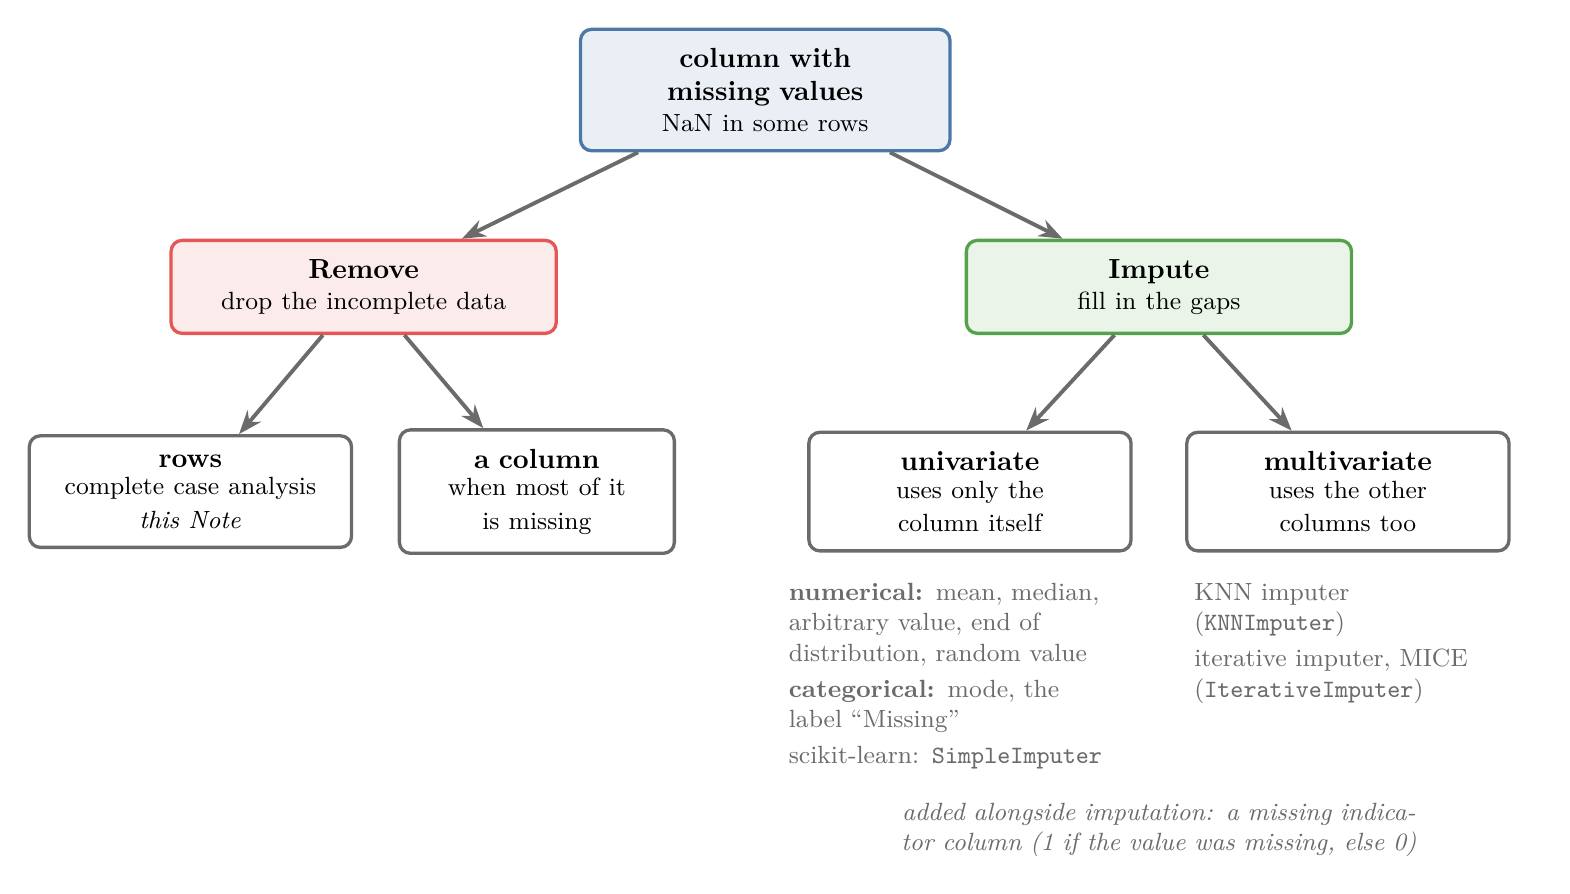
\begin{tikzpicture}
  \node[box=cblue, text width=4.2cm] (in) at (0,0) {\textbf{column with missing values}\\[-1pt]\small NaN in some rows};
  % two options
  \node[box=cred, text width=4.4cm] (rem) at (-5.1,-2.5) {\textbf{Remove}\\[-1pt]\small drop the incomplete data};
  \node[box=cgreen, text width=4.4cm] (imp) at (5,-2.5) {\textbf{Impute}\\[-1pt]\small fill in the gaps};
  \draw[arrow] (in) -- (rem);
  \draw[arrow] (in) -- (imp);
  % remove
  \node[box=cgrey, fill=white, text width=3.6cm] (cca) at (-7.3,-5.1) {\textbf{rows}\\[-1pt]\small complete case analysis\\ \textit{this Note}};
  \node[box=cgrey, fill=white, text width=3.0cm] (col) at (-2.9,-5.1) {\textbf{a column}\\[-1pt]\small when most of it\\ is missing};
  \draw[arrow] (rem) -- (cca);
  \draw[arrow] (rem) -- (col);
  % impute
  \node[box=cgrey, fill=white, text width=3.6cm] (uni) at (2.6,-5.1) {\textbf{univariate}\\[-1pt]\small uses only the\\ column itself};
  \node[box=cgrey, fill=white, text width=3.6cm] (mul) at (7.4,-5.1) {\textbf{multivariate}\\[-1pt]\small uses the other\\ columns too};
  \draw[arrow] (imp) -- (uni);
  \draw[arrow] (imp) -- (mul);
  \node[note, below=0.25cm of uni, text width=4.6cm, align=left] {\textbf{numerical:} mean, median,\\ arbitrary value, end of\\ distribution, random value\\[2pt] \textbf{categorical:} mode, the\\ label ``Missing''\\[2pt] scikit-learn: \texttt{SimpleImputer}};
  \node[note, below=0.25cm of mul, text width=3.9cm, align=left] {KNN imputer\\ (\texttt{KNNImputer})\\[2pt] iterative imputer, MICE\\ (\texttt{IterativeImputer})};
  \node[note, font=\sffamily\small\itshape, text width=9.5cm] at (5,-9.4) {added alongside imputation: a missing indicator column (1 if the value was missing, else 0)};
\end{tikzpicture}
\end{document}
